\documentclass{article}

\usepackage{amsmath, graphicx, tikz}


\begin{document}

Given $f, g\in L^{p}(\mu)$, and we investigate
$$
\phi(t)=\int_X|f+t g|^p \;d \mu.
$$

One can expect that $\Phi(t)$ is differentiable becasuse the integrand is continuous. First, let me give an example
$$
\phi(t)=\int_{0}^{2\pi}|\sin(x)+t \cos(x)|^2 \;d \mu,
$$
which is illustrated in the following figure.

\begin{figure}[ht]
    \centering
    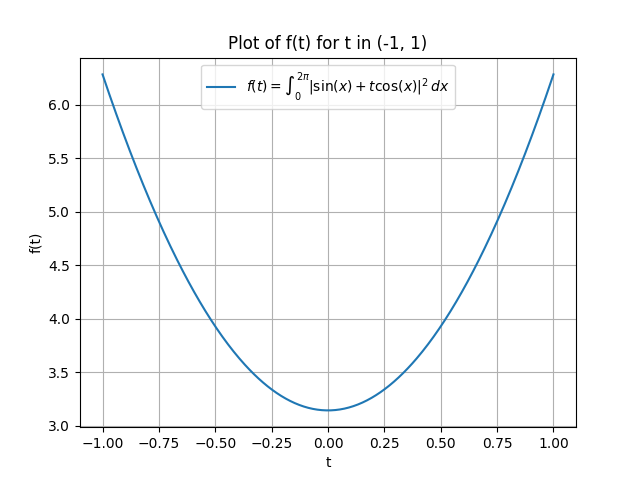
\includegraphics[width=0.75\textwidth]{Figure_1.png}
    \caption{}
    \label{fig:my_label}
\end{figure}

To prove this theoretically, we take $t=0$ as example
$$
\begin{aligned}
\phi^{\prime}(0)=& \lim _{t \rightarrow 0} \frac{\int_{X}|f+tg|^{p}-|f|^{p}}{t} \\
&= \int_{X} \lim _{t \rightarrow 0} \frac{|f+tg|^{p}-|f|^{p}}{t} \;d \mu.
\end{aligned}
$$
Notice that we need some convergence theorem to change the order of $\lim_{t\to 0}$ and $\int_{X}$.

It's the convexity of $|a+bt|^{p},p\geq 1$ that make it available.
For $t\in(-0.5,0.5)$, we have 
$$
\frac{|f+tg|^{p}-|f|^{p}}{t} \leq \frac{|f+g|^{p}-|f|^{p}}{1-0} = |f+g|^{p}-|f|^{p}.
$$
and it's easy to see that $|f+g|^{p}-|f|^{p}\in L^{1}(\mu)$ by the simple inequality $|a+b|^{p}\leq 2^{p-1}(|a|^{p}+|b|^{p})$.

Hence we apply L Hospital's rule to get
$$
\phi^{\prime}(0)=p \int_X|f|^{p-2} f g \;d \mu .
$$


\paragraph{Convex function.}
Here I wanna write something about convex function. 
 \begin{itemize}
\item The simplest convex function which is not differentiable is $|x|$.  More generally, a convex function can consist of connected line segments, also known as a piecewise linear function.
Interestingly, we can obtain such a function by connecting the tangent lines of a convex function or
connecting the points $(x_{i},f(x_{i}))$ where $f$ is convex.
\end{itemize}

\end{document}